\section[转动惯量]{\makebox[5em][s]{转动惯量}}\label{sec:09.04}

我们已经知道,质点的角动量为 $ \vec{ l } = \vec{ r } \times \vec{ p }$ ,它遵循的方程为
\begin{equation}\label{eqn:09.04.01}
  \frac { \dif \vec{l} } { \dif t } = \vec{M}
\end{equation}
如果质点在一个平面内运动,取此平面内某一点$ O $为原点(如图
\ref{fig:09.10}所示),则$ \vec{ r } $,$ \vec{ p } $总是在此平面内,由定义知,$ \vec{l} $总是垂直于此
平面的,故$ \vec{M} $也只能总是垂直于此平面,否则$ \vec{l} $的方向将变化,运动
% 275.jpg
\clearpage\noindent
就不可能是平面的。因此,在平面运动的情况\lhbrak 式\eqref{eqn:09.04.01}\rhbrak 可
写为标量形式
\begin{equation}\label{eqn:09.04.02}
  \frac { \dif l } { \dif t } = M
\end{equation}
\begin{wrapfigure}[6]{r}{11em}
  \centering
  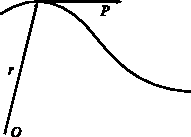
\includegraphics{figure/fig09.10}
  \caption{平面运动中的$ r $及$ p $}
  \label{fig:09.10}
\end{wrapfigure}
再进一步简化,假定质点绕中心$ O $作
半径为$ r $的圆周运动,则有$ l = m r v $,
或者$ l = m r ^ { 2 } \omega $,这里$ \omega = v / r $ 为角速率。
这样,式\eqref{eqn:09.04.02}可化为
\begin{equation*}
  \frac { \dif } { \dif t } \left( m r ^ { 2 } \omega \right) = M
\end{equation*}
由于$ m $,$ r $都是常数,所以
\begin{equation}\label{eqn:09.04.03}
  m r ^ { 2 } \frac { \dif \omega } { \dif t } = M
\end{equation}
式\eqref{eqn:09.04.03}是圆周运动的基本方程,它与一维运动中的质点的动
力学基本方程$ m \dfrac { \dif v } { \dif t } = F $ 很相似。这里,$ M $与$ F $的地位相当;$ m r ^ 2 $

\begin{wrapfigure}[9]{l}{13em}
  \centering
  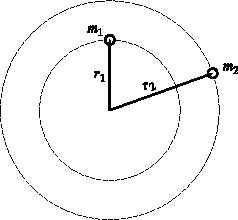
\includegraphics{figure/fig09.11}
  \caption{两质点的圆周运动}
  \label{fig:09.11}
\end{wrapfigure}
\noindent 与$ m $的地位相当。我们知道质量
$ m $是惯性的度量,在同样力$ F $的
作用下,质量$ m $越大,越不易于
加速。$ mr^2 $也有类似性质,在同
样的力矩$ M $作用下,$ mr^2 $越大,
角加速度越小。$ mr^2 $是关于转动
运动的惯性的度量,我们称它为
质点的转动惯量。

下面我们把转动惯量的概念
作些推广。首先讨论由质量为$ m_1 $,$ m _ 2 $的两个质点构成的体系,它
们在同一平面内绕同一中心作半径分别为$ r _ 1 $,$ r _ 2 $的圆周运动(图
\ref{fig:09.11}) 。它们的运动方程是:
% 276.jpg
\clearpage
{\setlength{\mathindent}{2em}
  \begin{align}
    \text{对} m _ 1 \text{有}\quad
    m _ { 1 } r _ 1 ^ { 2 } \frac { \dif \omega _ { 1 } } { \dif t } = M _ { 1 } \label{eqn:09.04.04} \\
    \text{对} m _ 2 \text{有}\quad
    m _ { 2 } r _ 2 ^ { 2 } \frac { \dif \omega _ { 2 } } { \dif t } = M _ { 2 } \label{eqn:09.04.05}
  \end{align}}%
式中 $ M _ { 1 } $ 、$ M _ { 2 } $分别是质点$ m _ 1 $及$ m _ 2 $所受到的总力矩,既应包括外界
物体作用在体系中质点上的力矩,也应包括体系内质点间相互作
用的力矩。前者称为外力矩,后者称为内力矩。将式\eqref{eqn:09.04.04}和
式\eqref{eqn:09.04.05}相加,得
\begin{equation*}
  m _ { 1 } r _ { 1 } ^ { 2 } \frac { \dif \omega _ { 1 } } { \dif t } + m _ { 2 } r _ { 2 } ^ { 2 } \frac { \dif \omega _ { 2 } } { \dif t } = M _ { 1 } + M _ { 2 }
\end{equation*}
在牛顿第三定律成立的条件下,体系的内力矩相互抵消,总和应
为零,所以上式可写为
\begin{equation}\label{eqn:09.04.06}
  m _ { 1 } r _ 1 ^ { 2 } \frac { \dif \omega _ { 1 } } { \dif t } + m _ { 2 } r _ 2 ^ { 2 } \frac { \dif \omega _ { 2 } } { \dif t } = M _ { \text { 外 } }
\end{equation}
式中$ M _ { \text { 外 } } $是体系受到的总外力矩。

用类似的方法,可以把上述结果推广到多质点所构成的体
系,即有$ n $个质点都绕$ O $作圆周运动,则有
\begin{equation}\label{eqn:09.04.07}
  \sum _ { i = 1 } ^ { n } m _ i r _ i ^ { 2 } \dfrac { \dif \omega _ { i } } { \dif t } = M _ { \text { 外 } }
\end{equation}
\begin{wrapfigure}[8]{r}{11em}
  \centering
  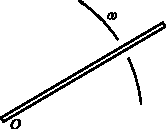
\includegraphics{figure/fig09.12}
  \caption{棒的转动}
  \label{fig:09.12}
\end{wrapfigure}
其中下标$ i = 1, 2, \dots, n $,指第$ i $个质
点的相应量。

上述体系中各质点的角速度可以
不相同。在特殊情况下,体系中各质
点的角速度可能都相同。譬如一根棒
子绕端点在一平面内转动(图\ref{fig:09.12}),
我们可以把棒看成许多质点的集合,
各质点的角速度相同,即
\begin{equation}\label{eqn:09.04.08}
  \omega _ { 1 } = \omega _ { 2 } = \cdots = \omega _ { n } = \omega
\end{equation}
% 277.jpg
我们把体系中各质点角速质不相等的情况,称为较差转动体系;
反之,称为刚性转动体系。对于较差转动,式\eqref{eqn:09.04.07}没有多少
用处,因为在一个方程中含有$ n $个变量,无法求解。要想求解,仍
必须回到$ n $个方程去。但对刚性转动,由式\eqref{eqn:09.04.08}可将式\eqref{eqn:09.04.07}简化为
\begin{equation*}
  \Big( \sum _ { i = 1 } ^ { n } m _ i r _ i ^ { 2 } \Big) \dfrac { \dif \omega } { \dif t } = M _ { \text { 外 } }
\end{equation*}
与式\eqref{eqn:09.04.03}对比,我们定义
\begin{equation}\label{eqn:09.04.09}
  I = \sum _ { i = 1 } ^ { n } m _ i r _ i ^ { 2 }
\end{equation}
称为刚性转动体系的对某一选定的转轴的转动惯量。这样,上述
方程就改写为
\begin{equation}\label{eqn:09.04.10}
  I \frac { \dif \omega } { \dif t } = M
\end{equation}
式\eqref{eqn:09.04.10}是刚性转动体系的动力学基本方程式,在不致引起误
解的情况下,我们可将$ M _ { \text { 外 } } $的下标去掉。

要强调指出:转动惯量与质量虽然都反映物体的惯性性质,
但二者有许多不同点。在牛顿力学中,质点的质量是不变的,对
任何运动都取该值;而转动惯量则取决于转动轴的位置,脱离确
定的转动轴,一般地谈论转动惯量是无意义的。

作为一个例子,我们求地球对自转轴的转动惯量。这里已经
不是平面问题,但我们可以把地球分成许多垂直于自转轴的薄
层,每一层仍是平面问题,然后迭加在一起,就是整个地球对自
转轴的转动惯量。

为计算方便,假定地球的质量密度是均匀的,其值为$ \rho $。我们
采用球极坐标(图\ref{fig:09.13}),则位于$ \left( r, \theta, \varphi \right) $的体积元为
\begin{equation*}
  \dif V = r ^ { 2 } \sin \theta \dif r \dif \theta \dif \varphi
\end{equation*}
这个体积元中的质量为

% 278.jpg
\begin{figure}[h]
  \centering
  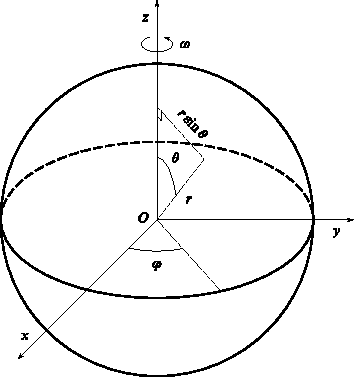
\includegraphics{figure/fig09.13}
  \caption{求地球的转动惯量}
  \label{fig:09.13}
\end{figure}
\begin{equation*}
  \begin{split}
    \dif m &= \rho \dif V \\
    &= \rho r ^ { 2 } \sin \theta \dif \theta \dif \varphi
  \end{split}
\end{equation*}
这个体积元到转轴的距离为$ r \sin \theta $,根据定义,它对自转轴的转动
惯量为$ \dif I = r ^ { 2 } \sin ^ { 2 } \theta \dif m $,所以整个地球对自转轴的转动惯量可由下
列积分求出:
\begin{equation*}
  \begin{split}
    I &= \int r ^ { 2 } \sin ^ { 2 } \theta \dif m \\
    &= \int _ 0 ^ { R } \int _ 0 ^ { \uppi } \int _ 0 ^ { 2 \uppi } \rho r ^ { 4 } \sin ^ { 3 } \theta \dif r \dif \theta \dif \varphi \\
    &= \frac { 8 \uppi } { 1 5 } \rho R ^ { 5 } \\
    &= \frac { 2 } { 5 } M _ { E } R ^ { 2 }
  \end{split}
\end{equation*}
其中$ R $为地球半径;$ M _ { E } = \dfrac { 4 \uppi } { 3 } R ^ { 3 } \rho $是地球的质量。将$ M _ { E } \approx
  % 279.jpg
  6 \times 1 0 ^ { 2 7 } $克, $ R \approx 6 \times 1 0 ^ { 3 } $公里代入,即求得
\begin{equation*}
  \begin{split}
    I _ { \text { 地 } } &= 8 \times 1 0 ^ { 40 } \text{ 克 }\! \cdot\!\!\text{ 米 } ^ 2 \\
    &= 8 \times 1 0 ^ { 37 } \text{ 公斤 }\! \cdot\!\! \text{ 米 } ^ 2
  \end{split}
\end{equation*}
